
%sudo apt-get install texlive-bibtex-extra
\documentclass{article}\usepackage[]{graphicx}\usepackage[]{color}
%% maxwidth is the original width if it is less than linewidth
%% otherwise use linewidth (to make sure the graphics do not exceed the margin)
\makeatletter
\def\maxwidth{ %
  \ifdim\Gin@nat@width>\linewidth
    \linewidth
  \else
    \Gin@nat@width
  \fi
}
\makeatother

\usepackage{Sweave}


\usepackage{float}
\usepackage{wrapfig}
\usepackage{hyperref}
\usepackage[backend=bibtex, style=nature, citestyle=authoryear]{biblatex}
\bibliography{WBVFM_IntroPar}
\newenvironment{knitrout}{}{}  %just a dummy environment
\makeatletter
\newcommand\gobblepars{%
    \@ifnextchar\par%
        {\expandafter\gobblepars\@gobble}%
        {}}
\makeatother



\title{A top-down approach to projecting the impacts of development aid on vegetative carbon sequestration}
\IfFileExists{upquote.sty}{\usepackage{upquote}}{}
\begin{document}
\begin{knitrout}


\maketitle






\begin{wrapfigure}[20]{r}{0.65\textwidth}\centering
%\begin{minipage}{.75\textwidth}
\begin{Schunk}

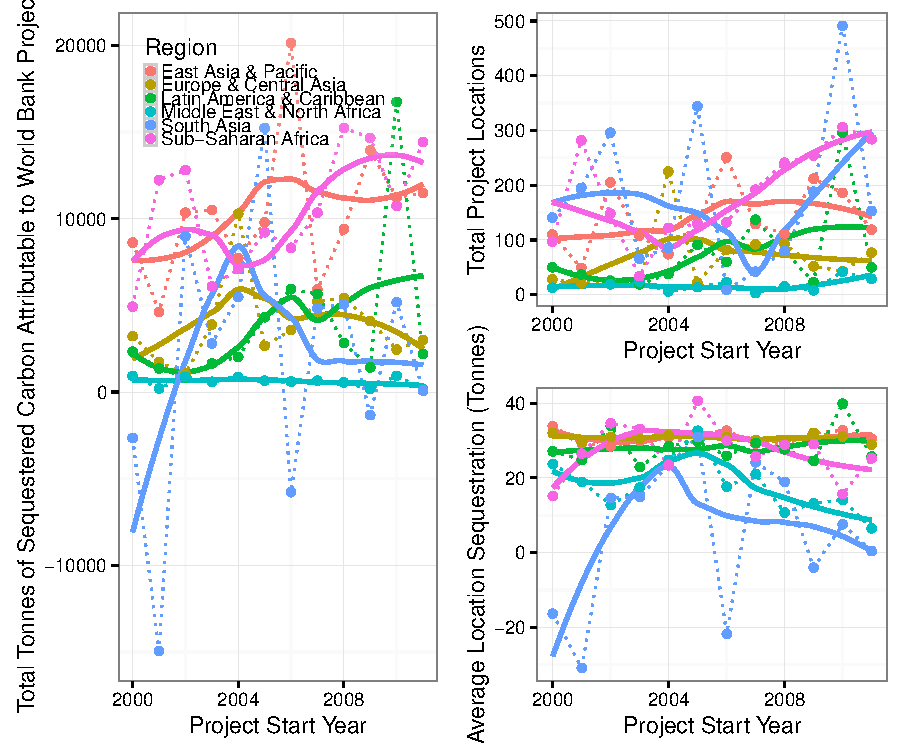
\includegraphics[width=\maxwidth]{figure/Fig1-1} \end{Schunk}
%\end{minipage}
\end{wrapfigure}  


  Since 1945, over \$4.9 trillion dollars of international aid has been allocated (\cite{tierney_more_2011}).
 To date there have been no estimates of the regional impact of this aid on the carbon cycle. \gobblepars

We apply a geographically weighted matching method (\cite{andam_measuring_2008}) to estimate the impact of World Bank projects implemented between 2000 and 2010 on sequestered carbon, using a novel, publically available double-blind coded dataset of 47,084 World Bank project locations \footnote{http://aiddata.org/level1/geocoded/worldbank}. \gobblepars

Considering only carbon sequestered due to fluctuations in vegetative biomass caused by World Bank projects, we conservatively estimate a global net positive increase in sequestration totaling 1,398,229 tonnes. 
Despite uncertainty in the global vegetative carbon stocks and flows (\cite{coulston_complex_2015}), we provide evidence of the success of environmental safeguards (\cite{laurance_reducing_2015}) implemented by the Bank in most regions over the last decade, and are able to highlight "bright spots" in time periods and regions which contained projects that enabled higher levels of carbon sequestration. 
In view of these analyses, we argue that subnational, geo-referenced data on the location of development finance and aid contains decision-relevant information for environmental policy.




\newpage
\printbibliography


%Summary Paragraph
%WB Global IE
%Runfola, Ben'Yishay, Tanner, Buchanan, Nagol
%Goodman, Trichler, Marty
%Acknowledge: Stewart, Kappel, Lu, Nicholson, Vijayan, Walter, Hild, Leu
\end{knitrout}
\end{document}
